\documentclass[border=15pt]{standalone}

\usepackage{ctex}

\usepackage{van-de-la-sehen}
\usepackage{van-le-trompe-loeil}

\newenvironment{rem}{\textbf{附注}\hspace{1em}}{}

\def\equals{=}

\begin{document}

\begin{minipage}{45cm}

\parbox{45cm}
{
    \textbf{各类元件}\vspace{1em}\\
    \begin{tabular}{cm{5cm}m{6cm}m{5cm}m{3cm}cm{5cm}m{6cm}m{5cm}m{5cm}}
        \toprule
        电阻 & %
        \begin{circuitikz}
            \draw (0,0) to[resistor,R=$R$,v=$u$,i=$i$] (3,0);
        \end{circuitikz} & %
        $\displaystyle \begin{aligned}
            & u = iR, \\
            & \+vZ = R
        \end{aligned}$ & & & OP & \begin{circuitikz} \draw
(0,0) node[op amp] (opamp) {} %
(opamp.+) node[left] {$u_+,i_+$} %
(opamp.-) node[left] {$u_-,i_-$} %
(opamp.out) node[right] {} %
;\end{circuitikz} & $\displaystyle \begin{aligned}
    & i_1 = i_2 = 0, \\
    & u_1 = u_2
\end{aligned}$ \\
        \midrule
        电容 & % 
        \begin{circuitikz}
            \draw (0,0) to[capacitor,C=$C$,v=$u$,i=$i$] (3,0);
        \end{circuitikz} & %
        $\displaystyle \begin{aligned}
            & i = C\+dtdu,\quad u = \rec{C}\int_{-\infty}^t i\pare{\xi}\,\rd{\xi}, \\
            & \+vZ = \rec{\+vj\omega C},\quad w = \half Cu^2
        \end{aligned}$ & %
        直流稳态\vspace{1em}\newline \begin{circuitikz}
            \draw (0,0) to[short, -o] (1,0) to[open,l=$u_{\infty}$] (2,0) to[short, o-] (3,0);
        \end{circuitikz} & $\displaystyle \begin{aligned}
             u &\leftrightarrow i \\
             C &\leftrightarrow L \\
             \+vZ &\leftrightarrow \+vY = \rec{\+vZ}
        \end{aligned}$ &%
        电感 & % 
        \begin{circuitikz}
            \draw (0,0) to[inductor,L=$L$,v=$u$,i=$i$] (3,0);
        \end{circuitikz} & %
        $\displaystyle \begin{aligned}
            & u = L\+dtdi,\quad i = \rec{L}\int_{-\infty}^t u\pare{\xi}\,\rd{\xi}, \\
            & \+vZ = \+vj\omega L,\quad w = \half Li^2
        \end{aligned}$ & %
        直流稳态\vspace{1em}\newline \begin{circuitikz}
            \draw (0,0) to[short, i=$i_\infty$] (3,0);
        \end{circuitikz} \\
        \midrule
        电压源 & % 
        \begin{circuitikz}
            \draw (0,0) to[european voltage source,v<=$U_s$] (3,0);
        \end{circuitikz} & %
        $\displaystyle \begin{aligned}
            u=U_s
        \end{aligned}$ & %
        置零\vspace{1em}\newline \begin{circuitikz}
            \draw (0,0) to[short] (3,0);
        \end{circuitikz} & & %
        电流源 & % 
        \begin{circuitikz}
            \draw (0,0) to[european current source,i=$I_s$] (3,0);
        \end{circuitikz} & %
        $\displaystyle \begin{aligned}
            i=I_s
        \end{aligned}$ & %
        置零\vspace{1em}\newline \begin{circuitikz}
            \draw (0,0) to[short, -o] (1,0) to[open] (2,0) to [short,o-] (3,0);
        \end{circuitikz} \\
        $\displaystyle \begin{aligned}
            \text{VCVS} \\
            \text{CCVS}
        \end{aligned}$ & % 
        \begin{circuitikz}
            \draw (0,0) to[european controlled voltage source,v<=$\mu u_1$,l_=$ri_1$] (3,0);
        \end{circuitikz} & %
        $\displaystyle \begin{aligned}
            u&=\mu u_1 \\
            u&=r i_1
        \end{aligned}$ & %
        N/A & &%
        $\displaystyle \begin{aligned}
            \text{CCCS} \\
            \text{VCCS}
        \end{aligned}$ & % 
        \begin{circuitikz}
            \draw (0,0) to[european controlled current source,i=$\alpha i_1$] (3,0);
            \draw (2.5,0) node[anchor=north] {$gu_1$};
        \end{circuitikz} & %
        $\displaystyle \begin{aligned}
            i&=\alpha i_1 \\
            i&=gu_1
        \end{aligned}$ & %
        N/A \\
        %CCVS & % 
        %\begin{circuitikz}
        %    \draw (0,0) to[european controlled voltage source,v<=$ri_1$] (3,0);
        %\end{circuitikz} & %
        %$\displaystyle \begin{aligned}
        %    u=ri_1
        %\end{aligned}$ & %
        %N/A & &%
        %VCCS & % 
        %\begin{circuitikz}
        %    \draw (0,0) to[european controlled current source,i=$gu_1$] (3,0);
        %\end{circuitikz} & %
        %$\displaystyle \begin{aligned}
        %    i=gu_1
        %\end{aligned}$ & %
        %N/A \\
        \bottomrule
    \end{tabular}
}
\vspace{0.5cm}
\newline
\parbox{45cm}
{
    \textbf{电路定理}\vspace{1em}\\
    \begin{tabular}{cm{8cm}m{7cm}ccm{8cm}m{9cm}}
        \toprule
        Kirchhoff电压定律 & %
        \begin{tikzpicture}[scale=0.5]
        \ctikzset{bipoles/length=.5cm}
            \draw (0:3) to[twoport,v=$u_1$] (60:3) to[twoport,v=$u_2$] (120:3) to[twoport,v=$\cdots$] (180:3) to[twoport,v=$\cdots$] (240:3) to[twoport,v=$\cdots$] (300:3) to[twoport,v=$u_n$] (360:3);
            \draw (0:3) to[short,*-] (0:4);
            \draw (60:3) to[short,*-] (60:4);
            \draw (120:3) to[short,*-] (120:4);
            \draw (180:3) to[short,*-] (180:4);
            \draw (240:3) to[short,*-] (240:4);
            \draw (300:3) to[short,*-] (300:4);
        \end{tikzpicture} & %
        $\displaystyle u_1 + u_2 + \cdots + u_n = 0 $ & %
        $\displaystyle \begin{aligned}
            u &\leftrightarrow i \\
            \text{回路} &\leftrightarrow \text{节点}
        \end{aligned}$ & %
        Kirchhoff电流定律 & %
        \begin{tikzpicture}
            \draw (0,0) to[short,i=$i_2$] (60:1.5);
            \draw (0,0) to[short,i=$\cdots$] (120:1.5);
            \draw (0,0) to[short,i=$\cdots$] (180:1.5);
            \draw (0,0) to[short,i=$\cdots$] (240:1.5);
            \draw (0,0) to[short,i=$i_n$] (300:1.5);
            \draw (0,0) to[short,*-,i=$i_1$] (0:1.5);
        \end{tikzpicture} & %
        $\displaystyle i_1 + i_2 + \cdots + i_n = 0 $ \\
        \midrule
        网孔分析 & %
        \begin{tikzpicture}
            \draw (0,0) to[european voltage source,v<=$u_{s1}$] (0,2) to[resistor,R=$R_1$,v=\mbox{}] (0,4) -- (2,4) to[resistor,invert,R=$R_3$,v=\mbox{}] (2,2) to[european voltage source,v_=$u_{s3}$] (2,0)  -- (0,0);
             \draw (2,0) to[short,*-] (4,0) to[european voltage source,v<=$u_{s2}$] (4,2) to[resistor,R=$R_2$,v=\mbox{}] (4,4) to[short,-*] (2,4);
            \draw[->] (0.8,1.7) arc (240:-60:0.5);
            \draw[->] (3.2,1.7) arc (-60:240:0.5);
            \draw (1,2) node {$i_{M1}$};
            \draw (3,2) node {$i_{M2}$};
        \end{tikzpicture} & %
        $\displaystyle \begin{aligned}
            &u_{s1} + i_{M1}R_1 + \pare{i_{M1} + i_{M2}}R_3 + u_{s3} = 0, \\
            &u_{s2} + i_{M2}R_2 + \pare{i_{M1} + i_{M2}}R_3 + u_{s3} = 0 \\
        \end{aligned} $ & %
        $\displaystyle \begin{aligned}
            i &\leftrightarrow u \\
            \text{回路} &\leftrightarrow \text{节点}
        \end{aligned}$ & %
        节点分析 & %
        \begin{tikzpicture}
            \draw (-90:1.5) to[resistor,R=$G_2$] (30:1.5) to[resistor,R=$G_3$] (150:1.5) to[resistor,R=$G_1$] (-90:1.5);
            \draw (-90:3) to[european current source,i=$i_{s2}$] (30:3) to[european current source,i<=$i_{s3}$] (150:3) to[european current source,i<=$i_{s1}$] (-90:3);
            \draw (-90:1.5) to[short,-*] (-90:3) (30:1.5) to[short,-*] (30:3) (150:1.5) to[short,-*] (150:3);
            \draw (30:3) node[anchor=north west] {$u_{N2}$};
            \draw (150:3) node[anchor=north east] {$u_{N1}$};
            \draw (-90:3) node[ground] {};
        \end{tikzpicture} & %
        $\displaystyle \begin{aligned}
            &i_{s1} - u_{N1}G_1 + \pare{-u_{N1} + u_{N2}}G_3 - i_{s3} = 0, \\
            &i_{s2} - u_{N2}G_2 + \pare{u_{N1} - u_{N2}}G_3 + i_{s3} = 0
        \end{aligned} $ \\
        \midrule
        叠加原理 & %
        \+:c5{m{26cm}}{\begin{circuitikz}
            \draw (0,0) to[european voltage source,v<=$u_S$,i=$i_1$, -*] (0,3) to[resistor,R=$R_1$,v=$u_1$, -*] (3,3) to[resistor,R=$R_2$,i=$i_2$,v=$u_2$, -*] (3,0) -- (0,0);
            \draw (3,0) -- (5,0) to[european current source,i=$i_S$] (5,3) -- (3,3);
        \end{circuitikz}\raisebox{1.5cm}{$\quad=\quad$}\begin{circuitikz}
            \draw (0,0) to[european voltage source,v<=$u_S$,i=$i_1'$, -*] (0,3) to[resistor,R=$R_1$,v=$u_1'$, -*] (3,3) to[resistor,R=$R_2$,i=$i_2'$,v=$u_2'$, -*] (3,0) -- (0,0);
            \draw (3,0) -- (5,0) to[short,-o] (5,1) to[open] (5,2) to[short,o-] (5,3) -- (3,3);
        \end{circuitikz}\raisebox{1.5cm}{$\quad+\quad$}\begin{circuitikz}
            \draw (0,0) to[short,i=$i_1''$] (0,3) to[resistor,R=$R_1$,v=$u_1''$, -*] (3,3) to[resistor,R=$R_2$,i=$i_2''$,v=$u_2''$, -*] (3,0) -- (0,0);
            \draw (3,0) -- (5,0) to[european current source,i=$i_S$] (5,3) -- (3,3);
        \end{circuitikz}} & %
        $\displaystyle \begin{aligned}
            i_k = i_k' + i_k'', \\
            u_k = u_k' + u_k''
        \end{aligned}$ \\
        \midrule
        置换定理 & %
        \+:c5{m{26cm}}{\begin{circuitikz}
            \draw (0,0) -- (2,0) -- (2,3) -- (0,3) -- (0,0);
            \draw (1,1.5) node {$N_1$};
            \draw (5,0) -- (7,0) -- (7,3) -- (5,3) -- (5,0);
            \draw (6,1.5) node {$N_2$};
            \draw (2,2.5) to[short,-o,i=$i\equals\beta$] (3.5,2.5) -- (5,2.5);
            \draw (2,0.5) to[short,-o] (3.5,0.5) -- (5,0.5);
            \draw (3.5,0.5) to[open,v<=$u\equals\alpha$] (3.5,2.5);
        \end{circuitikz}\raisebox{1.5cm}{$\quad=\quad$}\begin{circuitikz}
            \draw (0,0) -- (2,0) -- (2,3) -- (0,3) -- (0,0);
            \draw (1,1.5) node {$N_1$};
            \draw (2,2.5) to[short,-*,i=$\beta$] (3.5,2.5) to[european voltage source,v=$\alpha$,-*] (3.5,0.5) -- (2,0.5);
        \end{circuitikz}\raisebox{1.5cm}{$\quad=\quad$}\begin{circuitikz}
            \draw (0,0) -- (2,0) -- (2,3) -- (0,3) -- (0,0);
            \draw (1,1.5) node {$N_1$};
            \draw (2,2.5) to[short,-*] (3.5,2.5) to[european current source,i=$\beta$,-*,v<=$\alpha$] (3.5,0.5) -- (2,0.5);
        \end{circuitikz}} & %
        \parbox{8cm}{$N_1$中各支路电流电压不变 \begin{pitfall}
            注意电源极性.
        \end{pitfall}} \\
        \midrule
        串联 & %
        \begin{tikzpicture}
            \ctikzset{bipoles/length=1.0cm}
            \draw (0,0) to[resistor,l^=$R_1$,R=$R_1$] (1,0) to[resistor,l^=$R_2$,R=$R_2$] (2,0) to[resistor,l^=$\cdots$,R=$\cdots$] (3,0) to[resistor,l^=$R_n$,R=$R_n$] (4,0);
        \end{tikzpicture} & %
        $\displaystyle \begin{aligned}
            R = R_1 + R_2 + \cdots + R_n, \\
            \+vZ = \+vZ_1 + \+vZ_2 + \cdots + \+vZ_n
        \end{aligned}$ & %
        $\displaystyle \begin{aligned}
            \text{节点} & \leftrightarrow \text{回路} \\
            R & \leftrightarrow G
        \end{aligned}$ & %
        并联 & %
        \begin{tikzpicture}
             \ctikzset{bipoles/length=1.0cm}
             \draw (0,-0.5) -- (4,-0.5) (1,-0.5) to[resistor,R=$R_1$] (1,0.5) (2,-0.5) to[resistor,R=$R_2$](2,0.5) (3,-0.5) to[resistor,R=$\cdots$](3,0.5) (4,-0.5) to[resistor,R=$R_n$](4,0.5) (0,0.5) -- (4,0.5);
         \end{tikzpicture} & %
         $\displaystyle \begin{aligned}
             \rec{R} = \rec{R_1} + \rec{R_2} + \cdots + \rec{R_n}, \\
             \rec{\+vZ} = \rec{\+vZ_1} + \rec{\+vZ_2} + \cdots + \rec{\+vZ_n}
         \end{aligned}$ \\
        电压源串联 & %
        \begin{tikzpicture}
            \ctikzset{bipoles/length=1.0cm}
            \draw (0,0) to[european voltage source,v<=$u_{s1}$] (1,0) to[european voltage source,v<=$u_{s2}$] (2,0) to[european voltage source,v<=$\cdots$] (3,0) to[european voltage source,v<=$u_{sn}$] (4,0);
        \end{tikzpicture} & %
        $\displaystyle u_s = u_{s1} + u_{s2} + \cdots + u_{sn}$ & %
        $\displaystyle \begin{aligned}
            \text{节点} & \leftrightarrow \text{回路} \\
            \text{电压源} & \leftrightarrow \text{电流源}
        \end{aligned}$ & %
        电流源并联 & %
        \begin{tikzpicture}
             \ctikzset{bipoles/length=1.0cm}
             \draw (0,-0.5) -- (4,-0.5) (1,-0.5) to[european current source,i=$i_{s1}$] (1,1) (2,-0.5) to[european current source,i=$i_{s2}$](2,1) (3,-0.5) to[european current source,i=$\cdots$](3,1) (4,-0.5) to[european current source,i=$i_{sn}$](4,1) (0,1) -- (4,1);
         \end{tikzpicture} & %
         $\displaystyle i_{s} = i_{s1} + i_{s2} + \cdots + i_{sn}$ \\
        电压源并其它 & %
        \+:c2{m{10cm}}{%
        \hspace{-3cm}\begin{tikzpicture}
            \draw (0,0) to [european voltage source,v<=$u_s$] (0,2) (0,0) to[short,-*] (2,0) to[short,-o] (4,0) (0,2) to[short,-*] (2,2) to[short,-o] (4,2) (2,0) to[twoport] (2,2) (2,1) node {$N'$};
        \end{tikzpicture} \raisebox{1cm}{$\quad = \quad$} \begin{tikzpicture}
             \draw (0,0) to [european voltage source,v<=$u_s$] (0,2) (0,0) to[short,-o] (2,0) (0,2) to[short,-o] (2,2) (2,0) to[open] (2,2);
         \end{tikzpicture}
        } & $\displaystyle \begin{aligned}
            \text{回路} &\leftrightarrow \text{节点} \\
            \text{电压源} &\leftrightarrow \text{电流源}
        \end{aligned}$ & %
        电流源串其它 & %
        \+:c2{m{10cm}}{%
        \hspace{-3cm}
        \begin{tikzpicture}
            \draw (4,0) to[short,o-] (0,0) to[european current source,i=$i_s$] (0,2) to[twoport,-o] (4,2) (2,2) node {$N'$};
        \end{tikzpicture} \raisebox{1cm}{$\quad=\quad$} \begin{tikzpicture}
            \draw (2,0) to[short,o-] (0,0) to[european current source,i=$i_s$] (0,2) to[short,-o] (2,2);
        \end{tikzpicture}
        } %
        \\
        \midrule
        $\displaystyle \begin{array}{c}
            \text{Th\'evenin定理} \\
            \text{电压源串电阻}
        \end{array}$ & %
        \begin{tikzpicture}
            \draw (0,0) -- (2,0) -- (2,2) -- (0,2) -- (0,0) (1,1) node {$N$} (2,0.5) to[short,-o] (3,0.5) (2,1.5) to[short,-o] (3,1.5);
        \end{tikzpicture} \raisebox{1cm}{$\quad = \quad$} \begin{tikzpicture}
            \draw (2,0) to[short,o-] (0,0) to[european voltage source,v<=$u_{o}$] (0,2) to[resistor,R=$R_0$,-o] (2,2);
        \end{tikzpicture} & %
        $\displaystyle \begin{aligned}
            u_o &= \text{开路电压}, \\
            R_0 &= \text{独立源置零后等效电阻}
        \end{aligned}$ & $\displaystyle \begin{aligned}
            \text{电压源} &\leftrightarrow \text{电流源} \\
            R_0 &= R_0 \\
            u_o &= i_s R_0
        \end{aligned}$ & %
        $\displaystyle \begin{array}{c}
            \text{Norton定理} \\
            \text{电流源并电阻}
        \end{array}$ & \begin{tikzpicture}
            \draw (0,0) -- (2,0) -- (2,2) -- (0,2) -- (0,0) (1,1) node {$N$} (2,0.5) to[short,-o] (3,0.5) (2,1.5) to[short,-o] (3,1.5);
        \end{tikzpicture} \raisebox{1cm}{$\quad = \quad$} \begin{tikzpicture}
            \draw (2,0) to[short,o-] (0,0) to[european current source,i=$i_{s}$] (0,2) to[short,-o] (2,2) (1,0) to[resistor,l_=$R_0$, *-*] (1,2);
        \end{tikzpicture} & %
        $\displaystyle \begin{aligned}
            i_s &= \text{短路电流}, \\
            R_0 &= \text{独立源置零后等效电阻}
        \end{aligned}$  \\
        \midrule
        $\Delta\rightarrow Y$ & \begin{tikzpicture}
            \draw (-30:1.5) to[resistor,l_=$R_a$,*-*] (90:1.5) to [resistor,l_=$R_b$,*-*] (210:1.5) to[resistor,l_=$R_c$,*-*] (-30:1.5);
        \end{tikzpicture} \raisebox{1.125cm}{$\quad = \quad$} \begin{tikzpicture}
            \draw (0,0) to[resistor,R=$R_1$,*-*] (210:1.5) (0,0) to[resistor,R=$R_2$,*-*] (-30:1.5) (0,0) to[resistor,R=$R_3$,*-*] (90:1.5);
        \end{tikzpicture} & $\displaystyle \begin{aligned}
            R_1 &= \frac{R_bR_c}{R_a + R_b + R_c}, \\
            R_2 &= \frac{R_aR_c}{R_a + R_b + R_c}, \\
            R_3 &= \frac{R_aR_b}{R_a + R_b + R_c}
        \end{aligned}$ & $\displaystyle \begin{aligned}
            \text{节点}&\leftrightarrow\text{回路} \\
            R &\leftrightarrow G
        \end{aligned}$ & %
        $Y\rightarrow \Delta$ & %
        \begin{tikzpicture}
            \draw (0,0) to[resistor,R=$G_1$,*-*] (210:1.5) (0,0) to[resistor,R=$G_2$,*-*] (-30:1.5) (0,0) to[resistor,R=$G_3$,*-*] (90:1.5);
        \end{tikzpicture} \raisebox{1.125cm}{$\quad = \quad$} \begin{tikzpicture}
            \draw (-30:1.5) to[resistor,l_=$G_a$,*-*] (90:1.5) to [resistor,l_=$G_b$,*-*] (210:1.5) to[resistor,l_=$G_c$,*-*] (-30:1.5);
        \end{tikzpicture} & $\displaystyle \begin{aligned}
            G_a &= \frac{G_2G_3}{G_1 + G_2 + G_3}, \\
            G_b &= \frac{G_1G_3}{G_1 + G_2 + G_3}, \\
            G_c &= \frac{G_1G_2}{G_1 + G_2 + G_3}
        \end{aligned}$ \\
        \bottomrule
    \end{tabular}
}
\vspace{0.5cm}
\newline
\parbox{45cm}
{
    \textbf{动态电路}\vspace{1em}\\
    \begin{tabular}{cm{8cm}m{7cm}ccm{8cm}m{7cm}}
        \toprule
        RC电路 & \begin{tikzpicture}
            \draw (0,0) to[european voltage source,v<=$\stackrel{\displaystyle u_s\pare{t}}{\scriptstyle t\ge t_0}$] (0,2) to[resistor,R=$R$] (2,2) to[capacitor,v=$u_C$,i=$i_C$,C=$C$] (2,0) to[short] (0,0);
        \end{tikzpicture} & %
        $\displaystyle \begin{aligned}
            RC\+dtd{u_C} + u_C &= u_s\pare{t} \\
            \tau &= RC
        \end{aligned}$ & %
        $\displaystyle \begin{aligned}
            u_C &\leftrightarrow i_L \\
            C &\leftrightarrow L \\
            R &\leftrightarrow \rec{R}
        \end{aligned}$ & %
        RL电路 & %
        \begin{tikzpicture}
            \draw (0,0) to[european voltage source,v<=$\stackrel{\displaystyle u_s\pare{t}}{\scriptstyle t\ge t_0}$] (0,2) to[resistor,R=$R$] (2,2) to[inductor,v=$u_L$,i=$i_L$,L=$L$] (2,0) to[short] (0,0);
        \end{tikzpicture} & %
        $\displaystyle \begin{aligned}
            L \+dtd{i_L} + Ri_L &= u_s\pare{t} \\
            \tau &= \frac{L}{R}
        \end{aligned}$ \\
        \midrule
        三要素法 & \begin{tikzpicture}
            \draw (0,0) to[european voltage source,v<=$U_0\epsilon\pare{t}$] (0,3) -- (2,3) -- (2,2.5) (0,0) -- (2,0) -- (2,0.5) (1,0.5) -- (3,0.5) -- (3,2.5) -- (1,2.5) -- (1,0.5);
            \ctikzset{bipoles/length=0.6cm}
            \draw (3,2) -- (4,2) to[twoport,v^=$u_k\pare{t}$] (4,1) to[short,i=$i_k\pare{t}$] (3,1);
        \end{tikzpicture} & $\displaystyle \begin{aligned}
            & f\pare{t} =f\pare{\infty} + \brac{f\pare{0_+} - f\pare{\infty}}e^{-t/\tau} \\
            & R=\text{动态元件两端出去的等效电阻} \\
            & f\pare{t}\text{可以是}u_k\pare{t}\text{或}i_k\pare{t}
        \end{aligned}$ & \+:c3{m{7cm}}{%
            \parbox{7cm}{%
            \begin{pitfall}
                除了$u_C\pare{0_-} = u_C\pare{0_+}$和$i_L\pare{0_-} = i_L\pare{0_+}$, 一般的$f$不成立$f\pare{0_-}=f\pare{0_+}$.
            \end{pitfall}%
            }
        } & %
        \parbox{7cm}
        {
        \begin{rem}
        \mbox{}
            \begin{cenum}
                \item 设定$f\pare{\infty} = 0$得到零输入响应.
                \item 设定$f\pare{0_+} = 0$得到零状态响应.
                \item 三要素法的解本身是阶跃响应.
            \end{cenum}
        \end{rem}
        }
         %
        \\
        \midrule
        RLC电路 & %
        \begin{tikzpicture}
            \draw (0,0) to[european voltage source,v<=$\stackrel{\displaystyle u_s\pare{t}}{\scriptstyle t\ge t_0}$] (0,2) to[resistor,R=$R$] (2,2) to[inductor,i=$i_L$] (4,2) to[capacitor,v=$u_C$,C=$C$] (4,0) to[short] (0,0);
        \end{tikzpicture} & %
        $\displaystyle \begin{aligned}
            & LC \frac{\rd{^2u_C}}{\rd{t}} + RC\+dtd{u_C} + u_C = u_s\pare{t} \\
            & s_{1,2} = -\frac{R}{2L} \pm \sqrt{\pare{\frac{R}{2L}}^2 - \rec{LC}}
        \end{aligned}$ & $\begin{aligned}
            \text{串联} &\leftrightarrow \text{并联} \\
            u &\leftrightarrow i \\
            C &\leftrightarrow L \\
            R &\leftrightarrow G
        \end{aligned}$ & %
        GCL电路 & %
        \begin{tikzpicture}
            \draw (0,0) to[european current source,i=$\stackrel{\displaystyle i_s\pare{t}}{\scriptstyle t\ge t_0}$] (0,2) -- (2,2) to[resistor,R=$G$,*-*] (2,0) -- (0,0) (4,2) to[inductor,L=$L$,v=$u_L\pare{t}$,i=$i_L\pare{t}$,*-*] (4,0) (6,2) to[capacitor,C=$C$] (6,0) (2,2) -- (6,2) (2,0) -- (6,0);
        \end{tikzpicture} %
        & %
        $\displaystyle \begin{aligned}
            & LC\frac{\rd{^2i_L}}{\rd{t}} + GL\+dtd{i_L} + i_L = i_s\pare{t} \\
            & s_{1,2} = -\frac{G}{2C} \pm \sqrt{\pare{\frac{G}{2C}}^2 - \rec{LC}}
        \end{aligned}$ %
         \\
        \midrule
        过阻尼 & $\displaystyle \pare{\frac{R}{2L}}^2 > \rec{LC}$ & $\displaystyle u_{Ch}\pare{t} = K_1 e^{s_1 t} + K_2 e^{s_2t}$ & & 过阻尼 & $\displaystyle \pare{\frac{G}{2C}}^2 > \rec{LC}$ & $\displaystyle i_{Lh}\pare{t} = K_1 e^{s_1 t} + K_2 e^{s_2t}$ \\
        临界阻尼 & $\displaystyle \pare{\frac{R}{2L}}^2 = \rec{LC}$ & $\displaystyle u_{Ch}\pare{t} = \pare{K_1 + K_2 t}e^{st}$ & & 临界阻尼 & $\displaystyle \pare{\frac{G}{2C}}^2 = \rec{LC}$ & $\displaystyle i_{Lh}\pare{t} = \pare{K_1 + K_2t}e^{st}$ \\
        欠阻尼 & $\displaystyle \pare{\frac{R}{2L}}^2 < \rec{LC},\  \alpha = \frac{R}{2L}, \ \omega_d = \sqrt{\rec{LC} - \pare{\frac{R}{2L}}^2}$ & $\displaystyle u_{Ch}\pare{t} = e^{-\alpha t}\pare{K_1\cos\omega_d t + K_2\sin\omega_d t}$ & & 欠阻尼 & $\displaystyle \pare{\frac{G}{2C}}^2 < \rec{LC},\  \alpha = \frac{G}{2C}, \ \omega_d = \sqrt{\rec{LC} - \pare{\frac{G}{2C}}^2}$ & $\displaystyle i_{Lh}\pare{t} = e^{-\alpha t}\pare{K_1\cos\omega_d t + K_2\sin\omega_d t}$ \\
        \midrule
        RLC全响应 & %
        \begin{tikzpicture}
            \draw (0,0) to[european voltage source,v<=$U_s$] (0,2) to[resistor,R=$R$] (2,2) to[inductor,i=$i_L$] (4,2) to[capacitor,v=$u_C$,C=$C$] (4,0) to[short] (0,0);
        \end{tikzpicture} & %
        $\displaystyle \begin{aligned}
            & u_C\pare{t} = u_{Ch}\pare{t} + U_s \\
            & K_1\text{和}K_2\text{通过初始条件确定}
        \end{aligned}$ & & %
        GCL全响应 & %
        \begin{tikzpicture}
            \draw (0,0) to[european current source,i=$I_s$] (0,2) -- (2,2) to[resistor,R=$G$,*-*] (2,0) -- (0,0) (4,2) to[inductor,L=$L$,v=$u_L\pare{t}$,i=$i_L\pare{t}$,*-*] (4,0) (6,2) to[capacitor,C=$C$] (6,0) (2,2) -- (6,2) (2,0) -- (6,0);
        \end{tikzpicture} %
        & %
        $\displaystyle \begin{aligned}
            & i_L\pare{t} = i_{Lh}\pare{t} + I_s \\
            & K_1\text{和}K_2\text{通过初始条件确定}
        \end{aligned}$ %
         \\
        \midrule
        相量$\cos$ & \+:c2{m{15cm}}{%
        \parbox{30cm}{%
        $U_m\cos\pare{\omega t + \varphi_0} = U_m \angle\varphi_0=\ $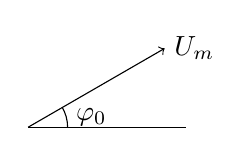
\begin{tikzpicture}
        \draw (0,0) -- (2,0);
        \draw[->] (0,0) -- (30:2);
        \draw (30:0.5) arc (30:0:0.5);
        \draw (15:0.5) node[anchor=west] {$\varphi_0$};
        \draw (30:2) node[anchor=west] {$U_m$};
        \end{tikzpicture}%
        }%
        } & & 相量$\sin$ & %
        %
        $\displaystyle U_m\sin\pare{\omega t + \varphi_0} = U_m \angle\pare{\varphi_0-\frac{\pi}{2}}=\ $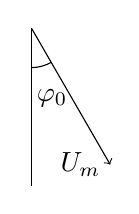
\begin{tikzpicture}
        \draw (0,0) -- (-90:2);
        \draw[->] (0,0) -- (-60:2);
        \draw (-60:0.5) arc (-60:-90:0.5);
        \draw (-68:0.7) node[anchor=north] {$\varphi_0$};
        \draw (-60:2) node[anchor=east] {$U_m$};
        \end{tikzpicture}%
        %
        & %
        \parbox{7cm}{%
        \begin{rem}
            将$u$替换为$\+vU$, $I$替换为$\+vI$, $R$替换为$\+vZ$, 则之前的电路定理仍然可直接适用得到正弦稳态结果.
        \end{rem}
        } \\
        \bottomrule
    \end{tabular}   
}

\end{minipage}

\end{document}
